\section{Experiments}
\label{sec:experiments}
We first describe the datasets we use and baseline methods we compare to, then present the results of \paperName{} for both object-level and scene-level novel view synthesis.


\subsection{Datasets}
\label{sec: exp_setup}
% Our experiments span both object and scene-level datasets. 
We train (and evaluate) \paperName{} on object-level and scene-level datasets separately.

\vspace{-1mm}
\textbf{Object-level Datasets. } We use the Objaverse dataset~\citep{deitke2023objaverse} to train \paperName{}. We follow the rendering settings in GS-LRM~\citep{zhang2024gslrmlargereconstructionmodel} and render 32 random views of $730$K objects. We test on two object-level datasets, Google Scanned Objects~\citep{downs2022gso} (GSO) and Amazon Berkeley Objects~\citep{collins2022abo} (ABO). 
GSO and ABO contain 1,099 and 1,000 objects, respectively. Following Instant3D~\citep{li2023instant3d} and GS-LRM~\citep{zhang2024gslrmlargereconstructionmodel}, we use 4 sparse views as test inputs and another 10 views as target images.

\vspace{-1mm}
\textbf{Scene-level Datasets. } We use the RealEstate10K dataset~\citep{realestate10k_zhou2018stereo}, which contains 80K video clips curated from 10K Youtube videos of both indoor and outdoor scenes. We follow the train/test data split used in pixelSplat~\citep{charatan2024pixelsplat}.

\vspace{-1mm}
\subsection{Training Details}
\label{sec: exp_details}
\vspace{-1mm}
\textbf{Improving Training Stability.} 
We observe that \paperName{} training crashes with plain transformer layers~\citep{vaswani2017transformer} due to exploding gradients.
% We observe the crash usually happens at the middle stage of training with gr
% adient explosion. 
We empirically find that using QK-Norm~\citep{henry2020qknorm} in the transformer layers stabilizes training.
This observation is consistent with \citet{bruce2024genie} and \citet{esser2024sd3}.
We also skip optimization steps with gradient norm > 5.0 in addition to the standard 1.0 gradient clipping.

%\vspace{-1mm}
\textbf{Efficient Training Techniques.} We use FlashAttention-v2~\citep{dao2023flashattention} in the xFormers~\citep{lefaudeux2022xformers}, gradient checkpointing~\citep{chen2016gradcheckpointing}, and mixed-precision training with Bfloat16 data type to accelerate training.

\vspace{-1mm}
\textbf{Other Details. } For more model and training details, please refer to Appendix~\ref{appendix:more_details}, and a detailed model architecture diagram (Fig.~\ref{fig:detailed_architecture}).


\definecolor{lightyellow}{rgb}{1,1, 0.8}
\definecolor{yellow}{rgb}{1,0.97, 0.65}
\definecolor{orange}{rgb}{1, 0.85, 0.7}
\definecolor{tablered}{rgb}{1, 0.7, 0.7}


\begin{table}[t!]
\caption{\small{
\textbf{Quantitative comparisons on object-level (left) and scene-level (right) view synthesis.}
For the object-level comparison, we matched the baseline settings with GS-LRM~\citep{zhang2024gslrmlargereconstructionmodel} in both input and rendering under both resolution of $256$ (Res-256) and $512$ (Res-512).
For the scene-level comparison, we use the same validation dataset used by pixelSplat~\citep{charatan2024pixelsplat}, which has $256$ resolution.
}
}
\vspace{-0.05in}
\begin{minipage}{.6\textwidth}
\resizebox{0.99\linewidth}{!}{
\begin{tabular}{r|ccc|ccc } 
    & \multicolumn{3}{c|} {ABO~\citep{collins2022abodatasetbenchmarksrealworld}} &  \multicolumn{3}{c} {GSO~\citep{downs2022gso}} \\ 
    & PSNR \(\uparrow\) & SSIM \(\uparrow\)  & LPIPS \(\downarrow\) & PSNR \(\uparrow\) & SSIM \(\uparrow\) & LPIPS \(\downarrow\) \\ 
    \midrule
    Triplane-LRM~\citep{li2023instant3d} (Res-512)  & \cellcolor{lightyellow}27.50 & \cellcolor{lightyellow}0.896  & \cellcolor{lightyellow}0.093 &  \cellcolor{lightyellow}26.54 & \cellcolor{lightyellow}0.893 & \cellcolor{lightyellow}0.064 \\
    GS-LRM~\citep{zhang2024gslrmlargereconstructionmodel} (Res-512)  &  \cellcolor{yellow}29.09  &  \cellcolor{orange}0.925 &  \cellcolor{yellow}0.085 & \cellcolor{orange}30.52 & \cellcolor{orange}0.952 & \cellcolor{orange}0.050  \\
    Ours Encoder-Decoder (Res-512) &   \cellcolor{orange}29.81 &   \cellcolor{yellow}0.913 &  \cellcolor{orange}0.065 &  \cellcolor{yellow}29.32 &  \cellcolor{yellow}0.933 &  \cellcolor{yellow}0.052   \\
    Ours Decoder-Only (Res-512) &  \cellcolor{tablered}32.10 &  \cellcolor{tablered}0.938 &  \cellcolor{tablered}0.045 &   \cellcolor{tablered}32.36  &   \cellcolor{tablered}0.962 &  \cellcolor{tablered}0.028  \\
    \midrule
    LGM~\citep{tang2024lgm} (Res-256) & \cellcolor{lightyellow}20.79 & \cellcolor{lightyellow}0.813  & \cellcolor{lightyellow}0.158 & \cellcolor{lightyellow}21.44  & \cellcolor{lightyellow}0.832 & \cellcolor{lightyellow}0.122 \\
    GS-LRM~\citep{zhang2024gslrmlargereconstructionmodel} (Res-256) &   \cellcolor{yellow}28.98  &  \cellcolor{orange}0.926 &  \cellcolor{yellow}0.074  &  \cellcolor{orange}29.59 &  \cellcolor{orange}0.944 &  \cellcolor{yellow}0.051 \\
    
     Ours Encoder-Decoder (Res-256)  &  \cellcolor{orange}30.35  &  \cellcolor{yellow}0.923 &  \cellcolor{orange}0.052 &  \cellcolor{yellow}29.19 &  \cellcolor{yellow}0.932 &  \cellcolor{orange}0.046 \\
     Ours Decoder-Only (Res-256)  & \cellcolor{tablered}32.47  &   \cellcolor{tablered}0.944 &  \cellcolor{tablered}0.037 &  \cellcolor{tablered}31.71 &  \cellcolor{tablered}0.957 &  \cellcolor{tablered}0.027  \\
\end{tabular}
}
\label{tab:compare_objects}
\hfill
\end{minipage}%
\begin{minipage}{.42\textwidth}
\resizebox{0.99\linewidth}{!}{
\begin{tabular}{r|ccc} 
    &  \multicolumn{3}{c}{RealEstate10k~\citep{realestate10k_zhou2018stereo}}  \\ 
    & PSNR \(\uparrow\) & SSIM \(\uparrow\)  & LPIPS \(\downarrow\)  \\ 
    \midrule
    pixelNeRF~\citep{yu2021pixelnerfneuralradiancefields} & 20.43 & 0.589  & 0.550 \\
    GPNR~\citep{suhail2022gpnr} & 24.11 & 0.793 &  0.255 \\
    Du et. al~\citep{du2023learningrendernovelviews} & 24.78 & 0.820  & 0.213 \\
    pixelSplat~\citep{charatan2024pixelsplat} & 26.09 & 0.863  & 0.136 \\
    MVSplat~\citep{chen2024mvsplatefficient3dgaussian} & \cellcolor{lightyellow}26.39 & \cellcolor{lightyellow}0.869  & \cellcolor{lightyellow}0.128 \\
    GS-LRM~\citep{zhang2024gslrmlargereconstructionmodel} & \cellcolor{yellow}28.10 & \cellcolor{yellow}0.892  & \cellcolor{yellow}0.114 \\
     Ours Encoder-Decoder  &  \cellcolor{orange}28.58 &   \cellcolor{orange}0.893 &  \cellcolor{orange}0.114  \\
     Ours Decoder-Only & \cellcolor{tablered}29.67 & \cellcolor{tablered}0.906 & \cellcolor{tablered}0.098 \\
\end{tabular}
}
\label{tab:compare_scenes}

\end{minipage}%
\vspace{-0.05in}
\end{table}










\subsection{Comparison to Baselines}
\label{sec: exp_result}
\begin{figure}[t]
    \centering
    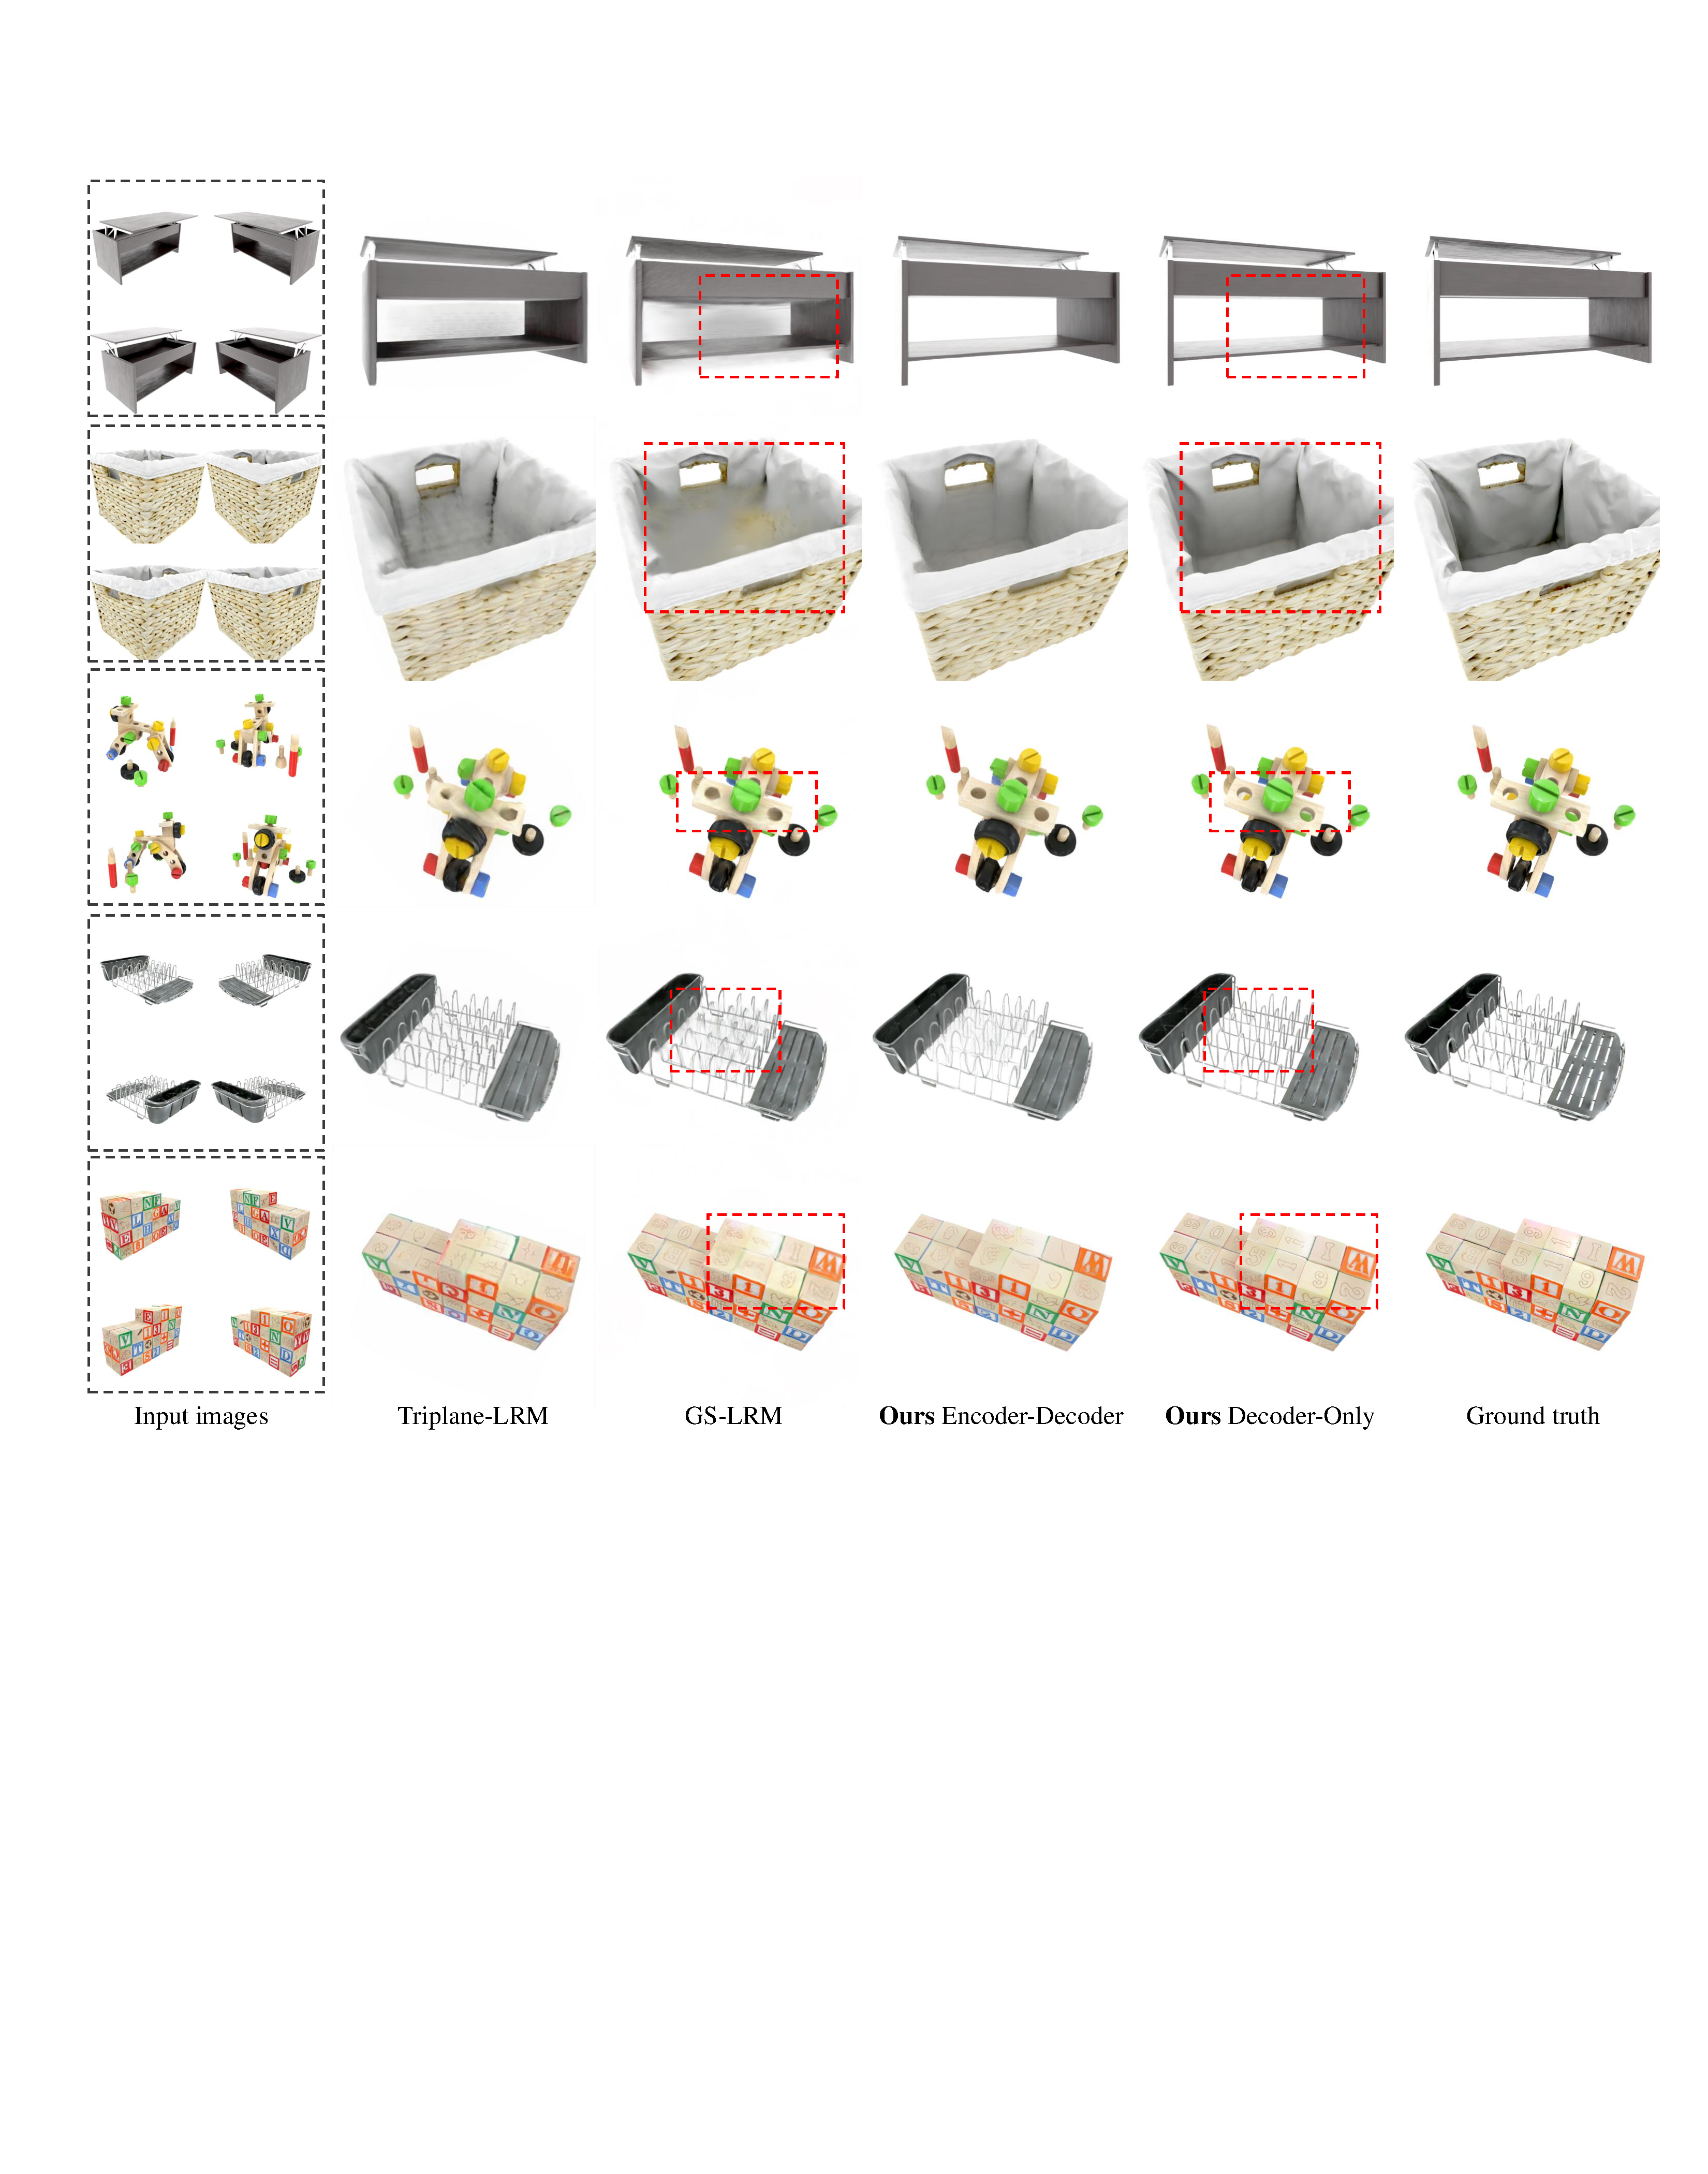
\includegraphics[width=0.95\textwidth]{./figures/object_comparison_512.pdf}
    \vspace{-0.6em}
    \caption{\small{
    \textbf{Object-level visual comparison at 512 resolution.} Given 4 sparse input posed images (leftmost column), we compare our high-res object-level novel-view rendering results with two baselines: Instant3D’s \textit{Triplane-LRM}~\citep{li2023instant3d} and \textit{GS-LRM} (Res-512)~\citep{zhang2024gslrmlargereconstructionmodel}. Both our Encoder-Decoder and Decoder-Only models exhibit fewer floaters (first example) and fewer blurry artifacts (second example), compared to the baselines. Our Decoder-Only model effectively handles complex geometry, including small holes (third example) and thin structures (fourth example). Additionally, it preserves high-frequency texture details (last example).
    }}
    \label{fig:highres_obj}
    \vspace{-0.1in}
\end{figure}
In this section, we describe our experimental setup and datasets (Sec.~\ref{sec: exp_setup}), introduce our model training details (Sec.~\ref{sec: exp_details}), report evaluation results (Sec.~\ref{sec: exp_result}) and perform an ablation study (Sec.~\ref{sec: exp_ablation}).

\vspace{-1mm}
\textbf{Object-Level Results.} We compare with Instant3D's Triplane-LRM~\citep{li2023instant3d} and GS-LRM~\citep{zhang2024gslrmlargereconstructionmodel} at a resolution of 512. As shown on the left side of Table~\ref{tab:compare_scenes}, our \paperName{} method achieves the best performance.
% against all prior works. 
In particular, at 512 resolution, our decoder-only \paperName{} achieves a 3 dB and 2.8 dB PSNR gain against the best prior method GS-LRM on ABO and GSO, respectively; our encoder-decoder \paperName{} achieves performance comparable to GS-LRM.

We also compare with LGM~\citep{tang2024lgm} at a resolution of 256, as the official LGM model is trained with that resolution. We also report the performance of models trained on resolution of 256. 
Compared with the best prior work GS-LRM, our decoder-only \paperName{} demonstrates a 3.5 dB and 2.2 dB PSNR gain on ABO and GSO, respectively; our encoder-decoder \paperName{} yields slightly better performance than GS-LRM.

These significant performance gains validate the effectiveness of our design target of removing 3D inductive bias. More interestingly, the larger performance gain on ABO suggests that \paperName can handle challenging materials, which are difficult for current handcrafted 3D representations. The qualitative results in Fig.~\ref{fig:highres_obj} and Fig.~\ref{fig:lowres_obj} also validate the high degree of realism of \paperName{}, especially for examples with specular materials, detailed textures, and thin, complex geometry. 

\begin{figure}[t]
    \centering
    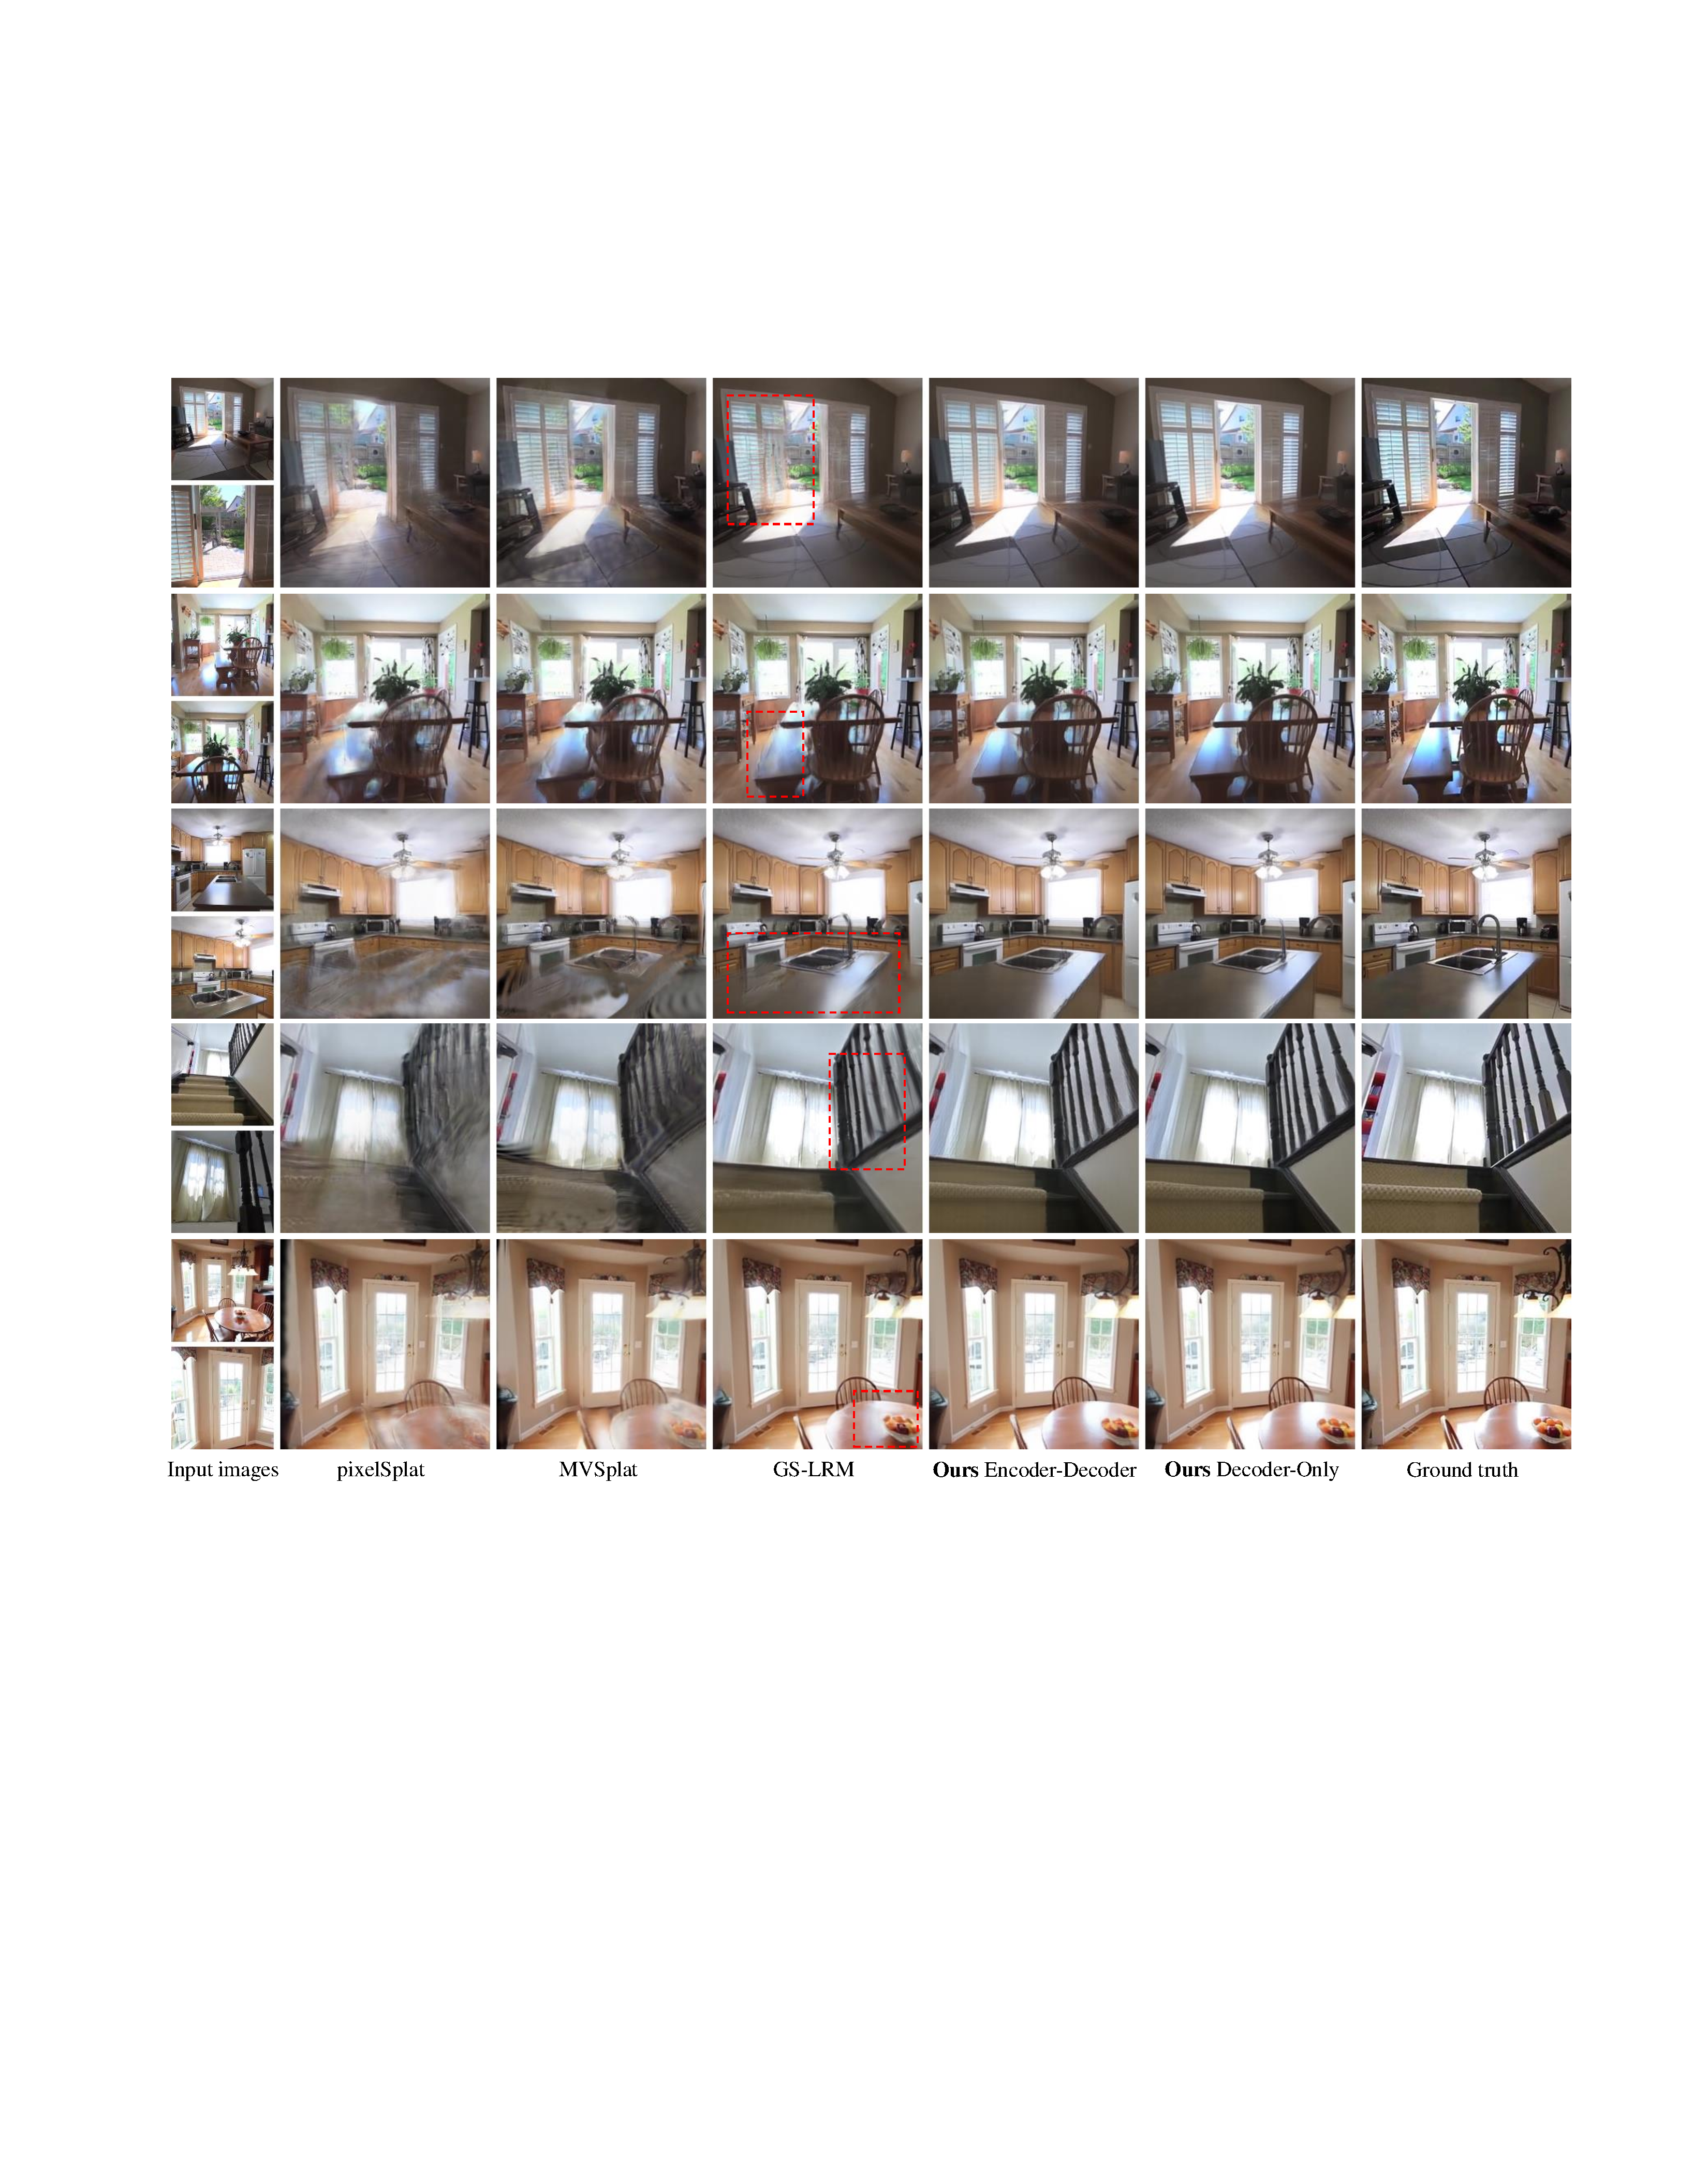
\includegraphics[width=\textwidth]{figures/scene_comparison_v2.pdf}
    \vspace{-5mm}
    \caption{\small{
    \textbf{Scene-level visual comparison.} We evaluate encoder-decoder and decoder-only  \paperName{} on scene-level view synthesis, comparing them to the prior leading baseline methods, namely pixelSplat~\citep{charatan2024pixelsplat}, MVSplat~\citep{chen2024mvsplatefficient3dgaussian}, and GS-LRM~\citep{zhang2024gslrmlargereconstructionmodel}. 
    Our results exhibit fewer texture and geometric artifacts, feature more realistic specular reflections, and are closer to the ground truth images.
    }
    } 
    \label{fig:scene_results}
    \vspace{-0.12in}
\end{figure}

\vspace{-1mm}
\textbf{Scene-Level Results.} We compare on scene-level inputs with 
% prior works 
pixelNeRF~\citep{yu2021pixelnerfneuralradiancefields}, GPNR~\citep{suhail2022gpnr}, ~\citet{du2023learningrendernovelviews}, pixelSplat~\citep{charatan2024pixelsplat}, MVSplat~\citep{chen2024mvsplatefficient3dgaussian} and GS-LRM~\citep{zhang2024gslrmlargereconstructionmodel}. As shown on the right side of Table~\ref{tab:compare_scenes}, our decoder-only \paperName{} shows a 1.6 dB PSNR gain compared with the best prior work, GS-LRM. Our encoder-decoder \paperName{} also demonstrates comparable results to GS-LRM. These improvements can be observed qualitatively in Fig.~\ref{fig:scene_results}, where \paperName{} has fewer floaters and better performance on thin structures and specular materials, consistent with the object-level results. These outcomes again validate the efficacy of our design of using minimal 3D inductive bias.



\vspace{-1mm}
\textbf{\paperName{} Trained with Only 1 GPU.} 
% We understand that the 
Limited computing is a key bottleneck for academic research. 
To show the potential of \paperName{} using academic-level resources, we train \paperName{} on the scene-level dataset~\citep{realestate10k_zhou2018stereo} following the setting of pixelSplat~\citep{charatan2024pixelsplat} and MVSplat~\citep{chen2024mvsplatefficient3dgaussian}, with only a single A100 80G GPU for 7 days. 
In this experiment, we use a smaller decoder-only model (denoted \paperName-small) with 6 transformer layers and a smaller batch size of 64 (in contrast to the default setting of 24 layers and batch size 512). 
Our decoder-only \paperName-small shows a performance of 27.66 dB PSNR, 0.870 SSIM, and 0.129 LPIPS. This performance surpasses the prior best 1-GPU-trained model, MVSplat, with a 1.3 dB PSNR gain. We also train a decoder-only \paperName (12 transformer layers, batch size 64) with 2 GPUs for 7 days, exhibiting a performance of 28.56 dB PSNR, 0.889 SSIM, and 0.112 LPIPS. This performance is even better than GS-LRM with 24 transformer layers trained on 64 GPUs.
These results show the promising potential of \paperName{} for academic research.



\vspace{-2mm}
\subsection{Ablation Studies}
\label{sec: exp_ablation}
\vspace{-1mm}
\textbf{Model Size.} In Tab.~\ref{table: abaltion_model_size}, we ablate the model size designs of both \paperName{} variants on both object and scene level. To save resources, these experiments are run with 8 GPUs and a total batch size of 64. 

For the encoder-decoder \paperName{}, we maintain the total number of transformer layers while allocating a different number of layers to the encoder and decoder. 
We observe that using more decoder layers helps performance while using more encoder layers harms performance. We hypothesize that this is because the encoder uses the latent representation to compress the input image information, and a deeper encoder makes this compression process harder to learn, resulting in greater compression errors.  
This observation suggests that using the inductive bias of the encoder and intermediate latent representation may not be optimal for the final quality, aligning with our observation that the decoder-only variant outperforms the encoder-decoder variant.


For the decoder-only \paperName{}, we experiment with using different numbers of transformer layers and model sizes in the decoder.
The experiment verifies that the decoder-only \paperName{} shows increasing performance when using more transformer layers, and validates the scalability of the decoder-only \paperName{}.

\begin{figure*}[t]
    \centering
    % \vspace{-2.5em}
    \begin{minipage}[t]{0.61\textwidth}
        \captionsetup{type=table}
        \setlength\tabcolsep{5pt}
        \centering
        %\vspace{-1.0em}
        \caption{\small{
        \textbf{Ablations studies on model sizes.} The following experiments are all run with 8 GPUs and a total batch size of 64.
        }}
        \resizebox{\textwidth}{!}{%
        \begin{tabular}{r|c|ccc|ccc} 
        %\toprule
        & & \multicolumn{3}{c}
        {GSO}
        &  \multicolumn{3}{c}{RealEstate10k}  \\ 
        & \# Params &PSNR \(\uparrow\) & SSIM \(\uparrow\)  & LPIPS \(\downarrow\)
        & PSNR \(\uparrow\) & SSIM \(\uparrow\)  & LPIPS \(\downarrow\) 
        \\ 
        \midrule
        Ours Encoder-Decoder  (6 + 18) & 173M &26.48 & 0.901 & 0.065 & 28.32 & 0.888 & 0.117  \\
        Ours Encoder-Decoder (12 + 12) & 173M &25.69 & 0.889 & 0.076 & 27.39 & 0.869 & 0.137 \\
        Ours Encoder-Decoder  (18 + 6) & 173M &24.74 & 0.873 & 0.091 & 26.80 & 0.855 & 0.152 \\
        \midrule
        Ours Decoder-Only (24 layers) & 171M & 27.04 & 0.910 & 0.055 & 28.89 & 0.894 & 0.108 \\
        Ours Decoder-Only (18 layers) & 128M &26.81 & 0.907 & 0.057 & 28.77 & 0.892 & 0.109 \\
        Ours Decoder-Only (12 layers) & 86M &26.11 & 0.896 & 0.065 & 28.61 & 0.890 & 0.111 \\
        Ours Decoder-Only (6 layers)  & 43M &24.15 & 0.865 & 0.092 & 27.62 & 0.869 & 0.129 \\
        %\bottomrule
        \end{tabular}
        }
        \label{table: abaltion_model_size}
    \end{minipage}
    \hfill
    \begin{minipage}[t]{0.37\textwidth}
        \captionsetup{type=table}
        \setlength\tabcolsep{5pt}
        \centering
        %\vspace{-1.0em}
        \caption{\small{
        \textbf{Ablations studies on model architecture.}
        }}
        \vspace{-0.15in}
        \resizebox{\textwidth}{!}{%
        \begin{tabular}{r|ccc} 
        %\toprule
        &  \multicolumn{3}{c}
        {GSO~\citep{downs2022gso}}  \\ 
        & PSNR \(\uparrow\) & SSIM \(\uparrow\)  & LPIPS \(\downarrow\)  \\ 
        \midrule
        Ours Encoder-Decoder & \textbf{28.07} & \textbf{0.920} & \textbf{0.053} \\
        Ours w/ CNN tokenizer & 27.59 & 0.914 & 0.052 \\
        Ours w/o latents' updating & 26.61 & 0.903 & 0.061  \\
        Ours w/ per-patch prediction & 26.27 & 0.897 & 0.072  \\
        Ours w/ pure cross-att decoder  & 24.60 & 0.876 & 0.085  \\
        \midrule
    &  \multicolumn{3}{c}{RealEstate10k~\citep{realestate10k_zhou2018stereo}}  \\ 
        & PSNR \(\uparrow\) & SSIM \(\uparrow\)  & LPIPS \(\downarrow\)  \\ 
        \midrule
        Ours Decoder-Only & \textbf{29.67} & \textbf{0.906} & \textbf{0.098} \\
        Ours w/ per-patch prediction & 28.98 & 0.897 & 0.103  \\
        %\bottomrule
        \end{tabular}
        }
        \label{table: ablation_model_arch}
    \end{minipage}
    \vspace{-0.5in}
\end{figure*}

\textbf{Model Architecture.} As shown in Tab.~\ref{table: ablation_model_arch}, we evaluate the effectiveness of our model designs. We also visualize the equivalent attention mask for each design in Fig.~\ref{fig:attention_mask} for better illustration. To save resources, the encoder-decoder experiments here are run with 32 GPUs, a total batch size of 256, and a decreased number of training target views of 8. The decoder-only experiment is run with our original setup.


Our encoder-decoder \paperName{} leverages an encoder to transform input images into a set of 1D tokens that serve as an intermediate latent representation of the 3D scene. 
A decoder can then render novel view images from this latent representation. While the encoder-decoder \paperName{} shares high-level conceptual similarities with SRT~\citep{sajjadi2022srt}---both are based on transformers and use 1D latent tokens as an intermediate latent representation without an explicit 3D representation---our encoder-decoder \paperName{} introduces a very distinct architecture that significantly enhances performance. In the following paragraphs, we evaluate many of our design decisions and also consider some alternate components based on SRT, showing that our design yields significant improvements.

\textbf{Tokenization Strategy for Encoder Input:} To generate input tokens for the encoder, we draw inspiration from ViT~\citep{dosovitskiy2020image} and recent LRMs~\citep{wei2024meshlrm,zhang2024gslrmlargereconstructionmodel}. 
Specifically, we tokenize the input images and their poses by simply splitting the concatenated input views and Plücker ray embeddings into non-overlapping patches. In contrast, SRT relies on shallow convolutional neural networks (CNNs) to extract patch features, which are then flattened into tokens. As an ablation study, we tried SRT's CNN-based tokenizing method and observed that it makes training more unstable with a larger grad norm, which leads to worse performance. As demonstrated in Tab.~\ref{table: ablation_model_arch}, replacing our simple tokenizer with SRT's CNN-based tokenizer degrades performance (ours w/ CNN tokenizer). 

\textbf{Fixed-Length Latent Encoding for Efficient Rendering:} Our encoder employs self-attention to progressively compress the information from posed input images into a fixed-length set of 1D latent tokens. This design ensures a consistent rendering speed, regardless of the number of input images, as shown in Fig.~\ref{fig: exp_increasing_views_fps}. This differs from approaches like SRT where latent token size increases linearly with input views, reducing rendering efficiency as the number of views grows.

\textbf{Bidirectional Self-Attention Decoder:}  The decoder of our encoder-decoder model utilizes pure (bidirectional) self-attention, allowing latent tokens and output target image tokens to attend to each other. This enables i) latent tokens to be updated by fusing information from themselves and from other tokens, which also means the parameters of the decoder are a part of the scene representation; ii) output patch pixels can also attend to other patches for joint updates, ensuring the global awareness of the rendered target image. We ablate our full-attention design choice by experimenting with different attention mechanisms, illustrated in Fig.~\ref{fig:attention_mask}. As shown in Tab.~\ref{table: ablation_model_arch}, disabling either the latents' updating (ours w/o latents' updating) or the joint updating of direct output pixel patches (ours w/ per-patch prediction) significantly degrades performance. SRT cannot support either mechanism because it employs a decoder with pure cross-attention.
We experiment with an LVSM variant by adopting SRT's decoder designs. As shown in Tab.~\ref{table: ablation_model_arch} (ours w/ pure cross-att decoder), this modification leads to reduced performance. 


The decoder-only \paperName{} further pushes towards eliminating inductive bias, bypassing an intermediate representation altogether. 
It adopts a single-stream transformer to directly convert the input multi-view tokens into target view tokens, treating view synthesis like a sequence-to-sequence translation task, which is fundamentally different from prior work. 
We ablate the importance of the joint prediction of target image patches in the decoder-only \paperName{}. We design a variant where the colors of each target pose patch are predicted independently, without applying self-attention across other target pose patches. We achieve this by letting each transformer layer's key and value matrices only consist of updated input image tokens, while both the updated input image tokens and target pose tokens form the query matrices. 
As shown on the bottom part of Tab.~\ref{table: ablation_model_arch}, this variant shows worse performance, with a 0.7 dB PSNR degradation. This result demonstrates the importance of using both input and target tokens as context tokens for information exchange using the simplest full self-attention transformer, which is consistent with our philosophy of reducing inductive bias.


\subsection{Discussion}


\begin{figure*}[t]

\vspace{-10mm}
    \centering
    \begin{minipage}[t]{0.48\textwidth}
        \centering
        \resizebox{\linewidth}{!}{
        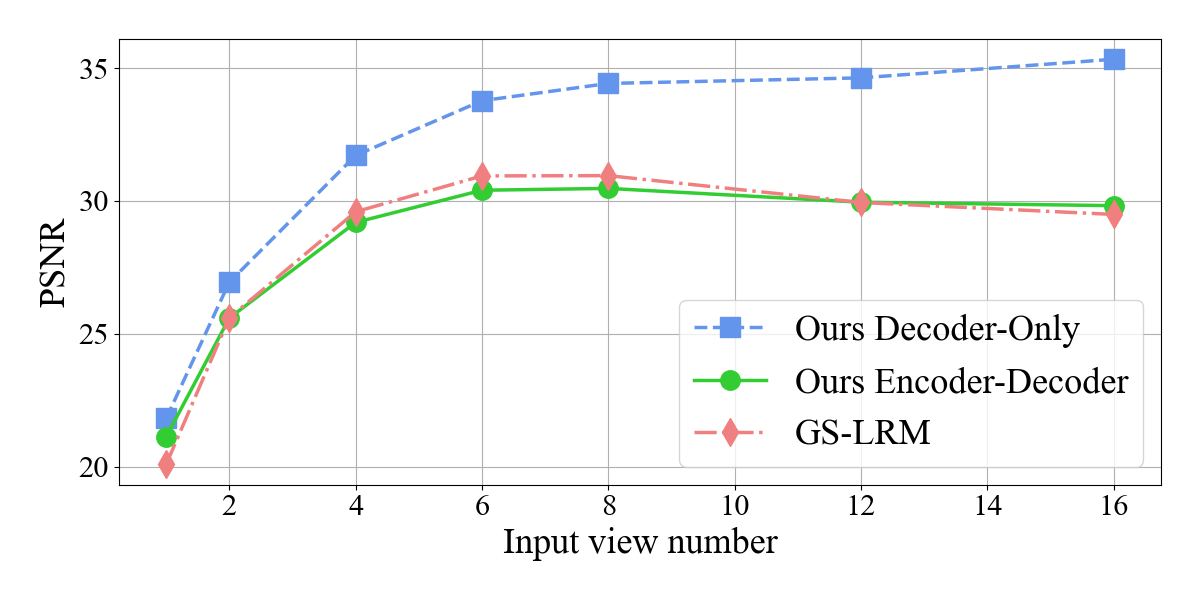
\includegraphics[width=\textwidth]{figures/NVS_PSNR_under_different_input_view_number_gso.png} % Use your file name here
        }
        \vspace{-0.3in}
        \caption{\small{\textbf{Zero-shot generalization to different number of input images} on the GSO dataset~\citep{downs2022gso}. We note that all models are trained with just 4 input views.}}
        \label{fig: exp_increasing_views}
         \vspace{-0.3in}
    \end{minipage}%
    % Subfigure for the table
    \hfill
    \begin{minipage}[t]{0.47\textwidth}
        \centering
        \resizebox{\linewidth}{!}{
        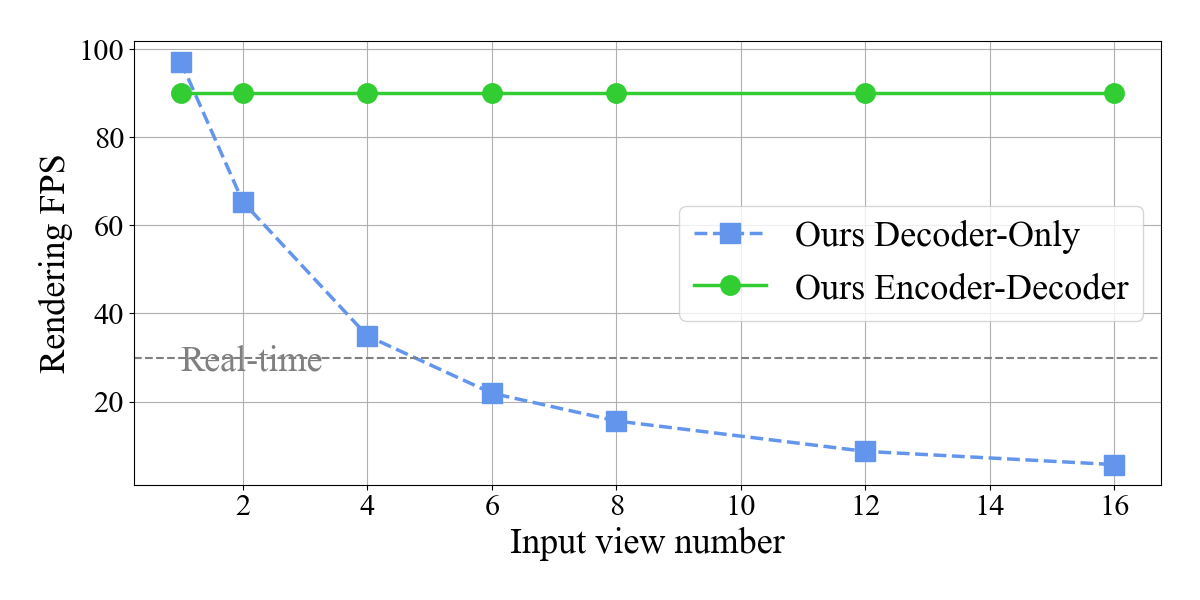
\includegraphics[width=\textwidth]{figures/NVS_PSNR_under_different_input_view_fps.png} % Use your file name here
        }
        \vspace{-0.3in}
        \caption{\small{\textbf{Rendering FPS with different number of input images.} We test the FPS on the object level under $256 \times 256$ resolution. We refer to rendering as the decoding process, which synthesizes novel views from latent tokens or input images.}}
        \label{fig: exp_increasing_views_fps}
    \end{minipage}%
    \vspace{-0.3in}
\end{figure*}


\vspace{-1mm}
\textbf{Zero-shot Generalization to More Input Views.} We compare our \paperName{} with GS-LRM by taking different numbers of input views during inference. 
We report the results on object-level inputs.
Note that these models are trained with 4 input views, and tested on varying numbers of input views in a zero-shot manner. 
As shown in Fig.~\ref{fig: exp_increasing_views}, our decoder-only \paperName{} shows increasingly better performance when using more input views, verifying the scalability of our model design at test time. Our encoder-decoder \paperName{} shows a similar pattern as GS-LRM, i.e., it exhibits a performance drop when using more than 8 input views. We conjecture that this is due to the inductive bias of the encoder-decoder design, i.e., using intermediate representation as a compression of input information limits performance. 
In addition, our single-input results (input view number = 1) are competitive and even outperform some of the baseline that takes 4 images as input.
These performance patterns validate our design target of using minimal 3D inductive bias for learning a fully data-driven rendering model and cohere with our discussion in Sec.~\ref{sec:method_model_archs}.

% \vspace{-1mm}
\textbf{Encoder-Decoder versus Decoder-Only.}
As mentioned in Sec.~\ref{Sec:Method}, the decoder-only and encoder-decoder architectures exhibit different trade-offs in speed, quality, and potential.

The encoder-decoder model transforms 2D image inputs into a fixed-length set of 1D latent tokens, which serve as a compressed representation of the 3D scene. This approach simplifies the decoder, reducing its model size. Furthermore, during the rendering/decoding process, the decoder always receives a fixed number of tokens, regardless of the number of input images, ensuring a consistent rendering speed. As a result, this model offers improved rendering efficiency, as shown in Fig.~\ref{fig: exp_increasing_views_fps}. Additionally, the use of 1D latent tokens as the latent representation for the 3D scene opens up the possibility of integrating this model with generative approaches for 3D content generation on its 1D latent space.
Nonetheless, the compression process can result in information loss, as the fixed latent token length is usually smaller than the original image token length, imposing an upper bound on performance. This characteristic of the encoder-decoder \paperName{} mirrors prior encoder-decoder LRMs; however, unlike those LRMs, our encoder-decoder \paperName{} does not have an explicit 3D structure.

In contrast, the decoder-only model learns a direct mapping from the input image to the target novel view, showcasing better scalability. 
For example, as the number of input images increases, the model can leverage all available information, resulting in improved novel view synthesis quality. 
However, this property also leads to a linear increase in input image tokens, leading to quadratic growth in computational complexity and limiting rendering speed.

% \vspace{-1mm}
\textbf{Single Input Image.} As shown in our project page, Fig.~\ref{fig:teaser} and Fig.~\ref{fig: exp_increasing_views}, we observe that our \paperName{} also works with a single input view for many cases, even though the model is trained with multi-view images during training. This observation shows the capability of \paperName{} to understand the 3D world, e.g., understanding depth, rather than performing purely pixel-level view interpolation.
 


